\documentclass[tikz,border=10pt]{standalone}
\usetikzlibrary{shapes.geometric, positioning, arrows.meta, scopes, patterns, shadows, calc}
% Assuming you have ez_utils defined, if not, remove the following line.
\usepackage{xstring}

\def\code#1{\color{olive}{\texttt{#1}}\color{black}~}
% \def\refer#1{Fig. \ref{#1}}
% \newcommand{\urlpath}[1]{%
% \begin{FVerbatim}[fontsize=\scriptsize]
% #1
% \end{FVerbatim}%
% }

\def\comment#1{\color{olive}{\textit{\% #1}} \color{black}}

\newcommand\ezeq[1]{$#1$}

\newcommand\ezcolumn[3]{
\begin{column}{#1\textwidth}
    \vspace{#2cm}
    #3
\end{column}
}

% \newenvironment{myenumerate}{%
%   \begin{enumerate}
%     \renewcommand{\theenumii}{\arabic{enumi}.\arabic{enumii}}
%   }
%   {%
%   \end{enumerate}
% }


\newcommand{\customenumerate}{%
  \renewcommand{\theenumii}{\arabic{enumi}.\arabic{enumii}}
  \renewcommand{\theenumiii}{\arabic{enumi}.\arabic{enumii}.\arabic{enumiii}}
}


\begin{document}
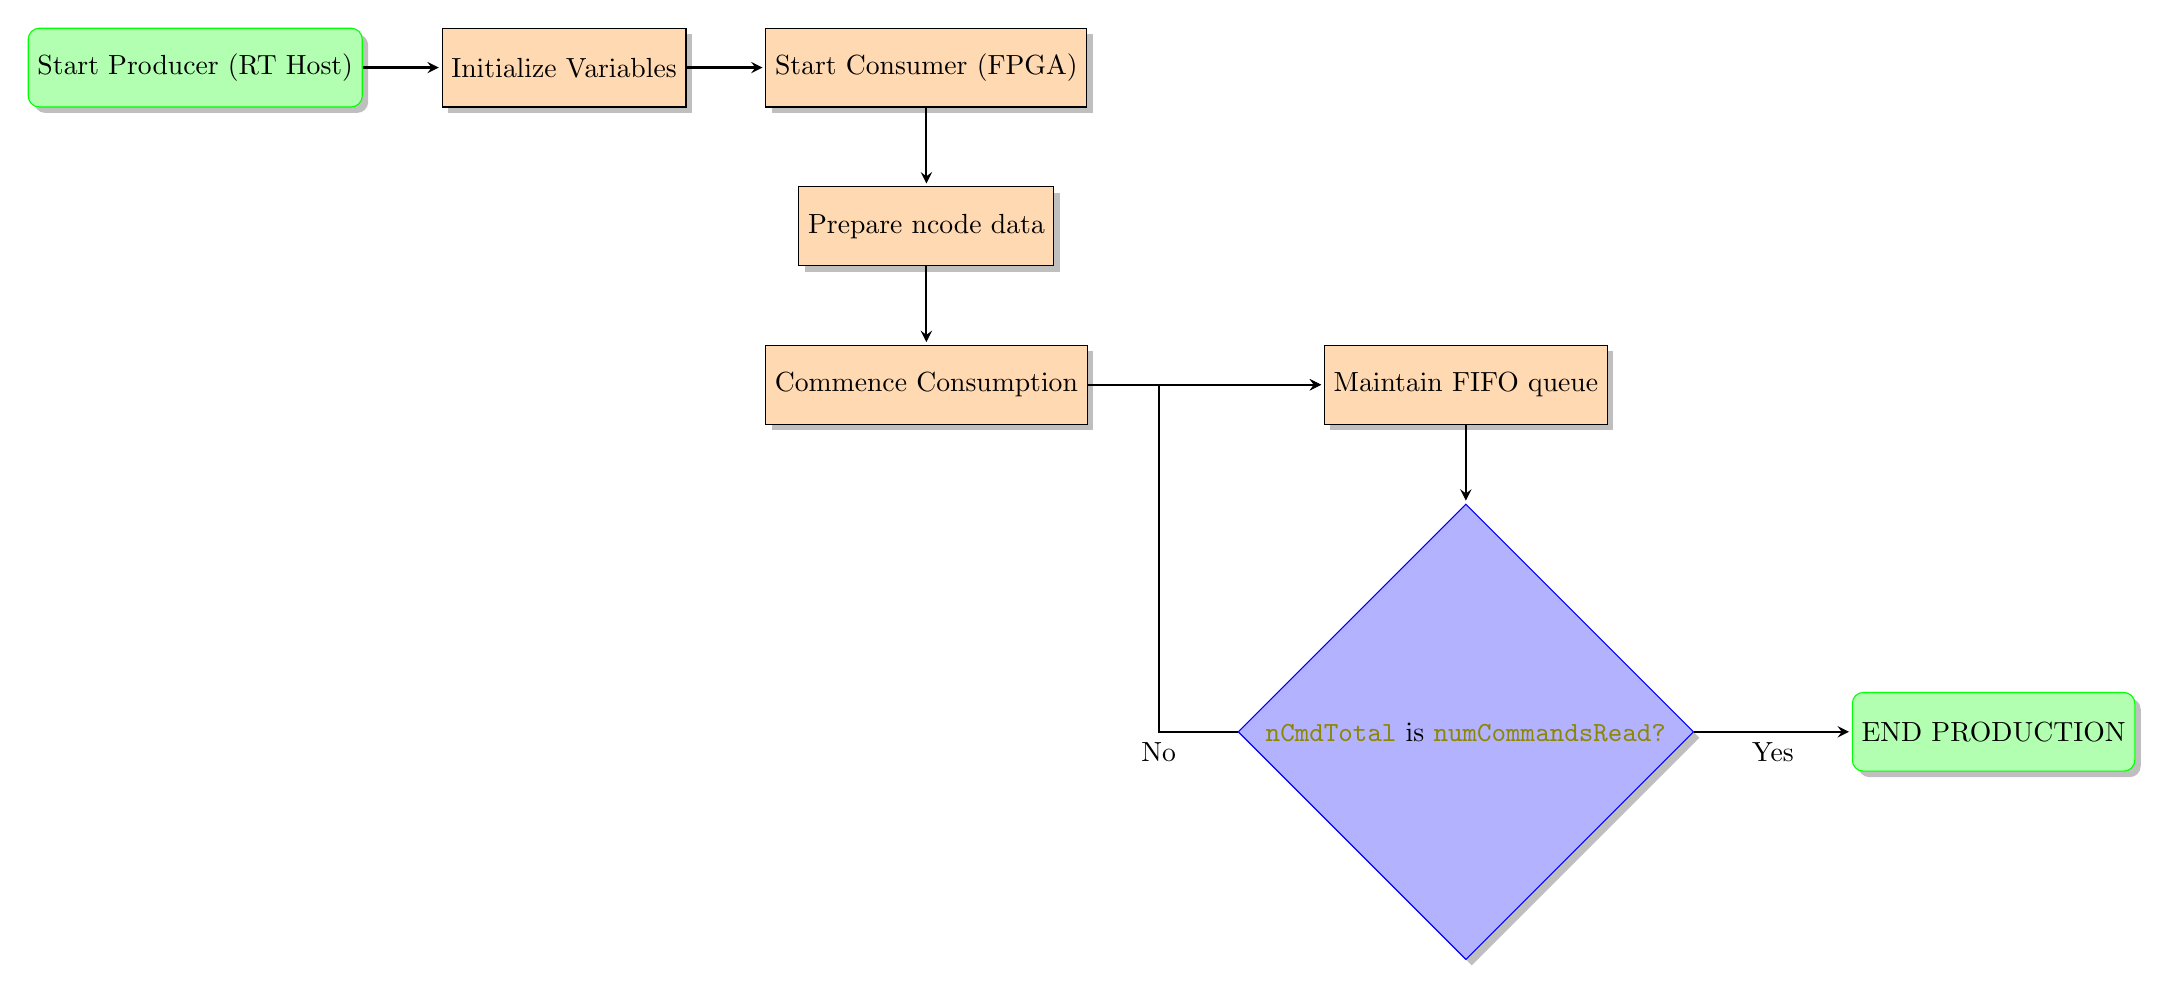
\begin{tikzpicture}[
    startstop/.style={rectangle, rounded corners, minimum width=3cm, minimum height=1cm, text centered, draw=green, fill=green!30, drop shadow},
    process/.style={rectangle, minimum width=3cm, minimum height=1cm, text centered, draw=black, fill=orange!30, drop shadow},
    io/.style={trapezium, trapezium left angle=70, trapezium right angle=110, minimum width=3cm, minimum height=1cm, text centered, draw=blue, fill=blue!30, drop shadow},
    decision/.style={diamond, minimum width=3cm, minimum height=1.5cm, text centered, draw=blue, fill=blue!30, drop shadow},
    arrow/.style={thick,->,>=stealth, shorten >=1pt},
]

% Nodes
\node[startstop] (start) {Start Producer (RT Host)};
\node[process, right=1cm of start] (init) {Initialize Variables};
\node[process, right=1cm of init] (startCons) {Start Consumer (FPGA)};
\node[process, below=1cm of startCons] (prepareData) {Prepare ncode data};
\node[process, below=1cm of prepareData] (commenceConsume) {Commence Consumption};
\node[process, right=3cm of commenceConsume] (maintainFIFO) {Maintain FIFO queue};
\node[decision, below=1cm of maintainFIFO] (loopDecision) {\code{nCmdTotal}is \code{numCommandsRead?}};
\node[startstop, right=2cm of loopDecision] (end) {END PRODUCTION};

% Connections using let...in for precise arrow drawing
\draw[arrow] (start) -- (init);
\draw[arrow] let \p1=(init.east), \p2=(startCons.west) in (\p1) -- (\p2);
\draw[arrow] (startCons) -- (prepareData);
\draw[arrow] let \p1=(prepareData.south), \p2=(commenceConsume.north) in (\p1) -- (\x1,\y2);
\draw[arrow] (commenceConsume) -- (maintainFIFO);
\draw[arrow] let \p1=(maintainFIFO.south), \p2=(loopDecision.north) in (\p1) -- (\x1,\y2);
\draw[arrow] (loopDecision) -- node[anchor=north] {Yes} (end);
\draw[arrow] (loopDecision.west) -| node[anchor=north] {No} ++(-1,0) |- (maintainFIFO.west);

\end{tikzpicture}
\end{document}
